\section{Dynamic Obstacles with Nav2 Navigation}
\label{sec:dynamic_obstacles_nav2}

To better approximate real-world navigation (where people and objects move), I added a custom ROS 2 package that spawns and animates dynamic obstacles in Gazebo while the robot navigates to a goal using Nav2.

\subsection{Implementation Overview}
The package \texttt{tb3\_nav2\_dynamic} provides:
\begin{itemize}
    \item \textbf{Dynamic obstacle node:} \texttt{dynamic\_obstacles\_node.py} spawns three box obstacles and moves them periodically.
    \item \textbf{Integrated launch:} \texttt{nav2\_dynamic.launch.py} can start Gazebo, Nav2 bringup, RViz2, an initial pose publisher, and the dynamic obstacle node.
\end{itemize}

The obstacles are created using \texttt{ros\_gz\_sim create} (SDF model) and moved using \texttt{ros\_gz\_sim set\_entity\_pose}. Each obstacle follows a simple trajectory (line or circle) parameterized by a center point, amplitude, and period. The update loop runs at \texttt{update\_rate\_hz} (default 2 Hz).

\subsection{How to Run}
\textbf{Prerequisite:} A saved map YAML from the SLAM section (e.g., \texttt{\$HOME/slam\_rl\_ws/maps/my\_map.yaml}).

\begin{bashcode}[title={Build \& Source the Workspace}]
cd ~/slam_rl_ws
colcon build --symlink-install
source install/setup.bash
\end{bashcode}

\begin{bashcode}[title={Launch Gazebo + Nav2 + RViz + Dynamic Obstacles}]
export TURTLEBOT3_MODEL=burger
ros2 launch tb3_nav2_dynamic nav2_dynamic.launch.py \
  map:=$HOME/slam_rl_ws/maps/my_map.yaml \
  start_dynamic_obstacles:=true
\end{bashcode}

\textbf{Operation:} In RViz2, set \textbf{2D Pose Estimate} (if needed) and then send a \textbf{Nav2 Goal}. The planner/controller should re-plan around moving boxes while executing the path.

\begin{figure}[H]
    \centering
    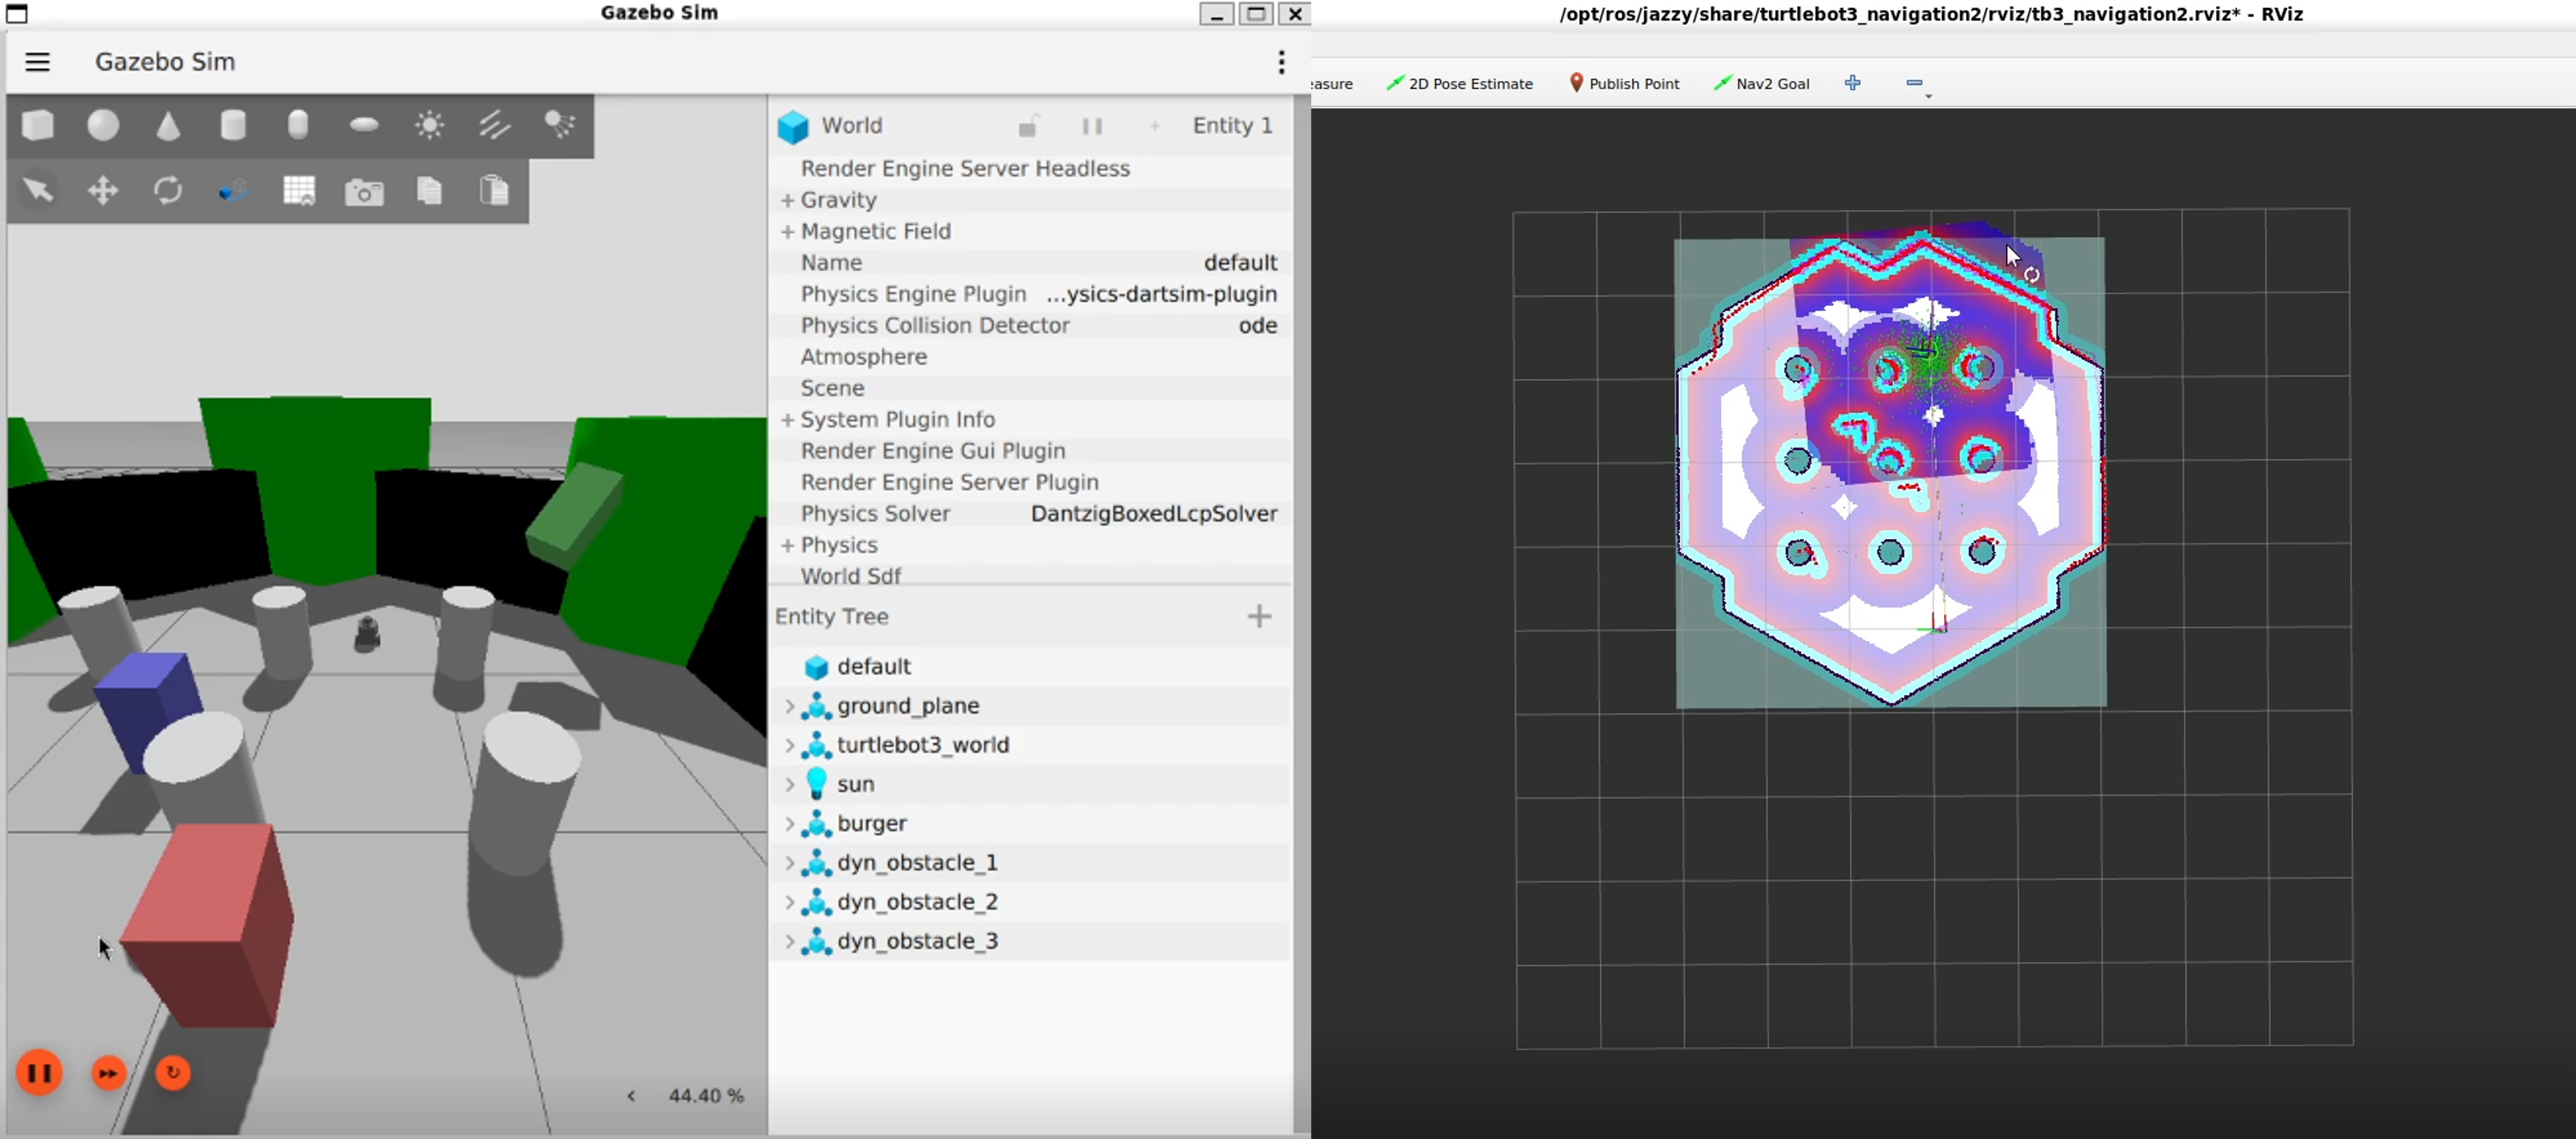
\includegraphics[width=0.9\linewidth]{images/moving_obj.png}
    \caption{Dynamic obstacles spawned and moved in Gazebo during Nav2 navigation.}
    \label{fig:moving_obj}
\end{figure}

\subsection{Notes}
\begin{itemize}
    \item If obstacles already exist in the world, set \texttt{spawn\_obstacles:=false} and only update poses.
    \item The trajectories and count of obstacles can be modified in \texttt{dynamic\_obstacles\_node.py}.
\end{itemize}
